\documentclass[tikz]{standalone}
\usepackage{tikz}
\usetikzlibrary{positioning, graphs}
\usetikzlibrary{graphs.standard}
\begin{document}
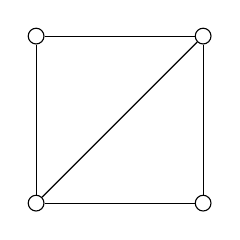
\begin{tikzpicture}
		[every node/.style={draw,circle,inner sep = 0mm, minimum size = 2mm}]
		\graph[clockwise, radius = 1.5cm, phase = 45, empty nodes]{subgraph C_n[n = 4, name = A]};
		
		\draw (A 1) -- (A 3);
\end{tikzpicture}
\end{document}